\chapter{多视角人脸数据采集平台}
\label{chap:platform}

在上一章的最后,本文提到了若要解决从单张图像同时重建人脸3D模型的几何和材质细节这一高度非适定的问题,则需要更多有关人脸的先验知识。
现有方法通常通过大量高精度的3D数据以训练神经网络模型来建模这种先验。
这些高精度的数据有时候以启发式的算法从2D图像中生成,
但更加鲁棒和贴近物理的方法自然是使用高精度的设备直接采集获得。

然而,可用于实现人脸几何和材质细节高精度重建的设备通常价格高昂,其采集的数据往往也由于商业价值较高而不被公开。
因此,不论是采集高精度的数据以重建高精度模型直接用于下游任务,还是用于建立先验以实现更高效的3D人脸重建,都离不开一套精准、高效、可靠的采集平台。

本章将介绍一套在较为有限的经济和时间成本下实现的多视角人脸数据采集平台。
该平台尽量使用可在市面上购买的部件,以减少对相关专业知识的需求。
同时配合一些定制的软件和硬件,实现对各个部件的高效统筹控制,为高精度重建所需的数据采集全流程提供支持。

\section{总体目标}

本文在设计和搭建该采集平台时,主要考虑了以下几个目标:
\begin{itemize}
\item 低硬件专业技能需求。本项目作为软件学院个人参与的项目,其所能得到的机械、结构、电子等方面的专业技术支持非常有限。
因此,为了能在有限的时间内完成该项目,本文尽可能地使用市面上可购买的部件,以减少对相关专业知识的需求。
虽然如此,本文还是使用了少量定制的硬件。

\item 高精度。高精度的数据是高精度3D重建的基础。
因此,对误差的控制贯穿与采集流程的各个环节,指导整个采集平台的软硬件设计。

\item 高效。整个平台在使用时,特别是在对被拍摄对象拍照时,应该尽可能地快速,以为大规模收集数据集提供可能。

\item 灵活。本平台作为一个主要用于研究性工作的采集平台,其需要具有一定的灵活性,以便应对研究中多变的需求。
基本地,该平台应能同时支持被动光源和主动光源的采集,能灵活配置相机和光源的位置和其他相关参数。

\item 可扩展。即使在本文写作完成后,该平台仍很可能被继续用于后续的研究工作。因此本平台也应适当考虑未来可能的更大规模的采集需求。

\end{itemize}

利用本平台采集的数据预计可用于多种3D人脸重建算法,例如本文其他部分介绍的基于可微分渲染的逆渲染方法。
同时也可用于如多目立体等传统的计算机视觉算法。

本章的主要贡献在于对该平台各个部分的设计和实现,以及对其性能的评估验证。
本章的剩余内容将具体介绍该平台的各个部分。

\section{整体结构设计}

本平台的硬件框架结构设计主要是参考了\citet{RiviereGBGB20}所展示的布局。
首批配置了12台相机和4台带有柔光箱的摄影灯,其中相机固定在3个铝型材搭建的、定制的、高自由度可调节的支架上。
灯则由于其体积质量较大,且市面上缺少相应的单独连接件产品,无法稳固地固定在支架上,因此直接使用了单独的专用灯架固定,以确保安全。
图\ref{fig:HDRI}展示了该平台硬件的整体布局。

\begin{figure}
\centering
\begin{subfigure}[b]{0.3\textwidth}
    \centering
    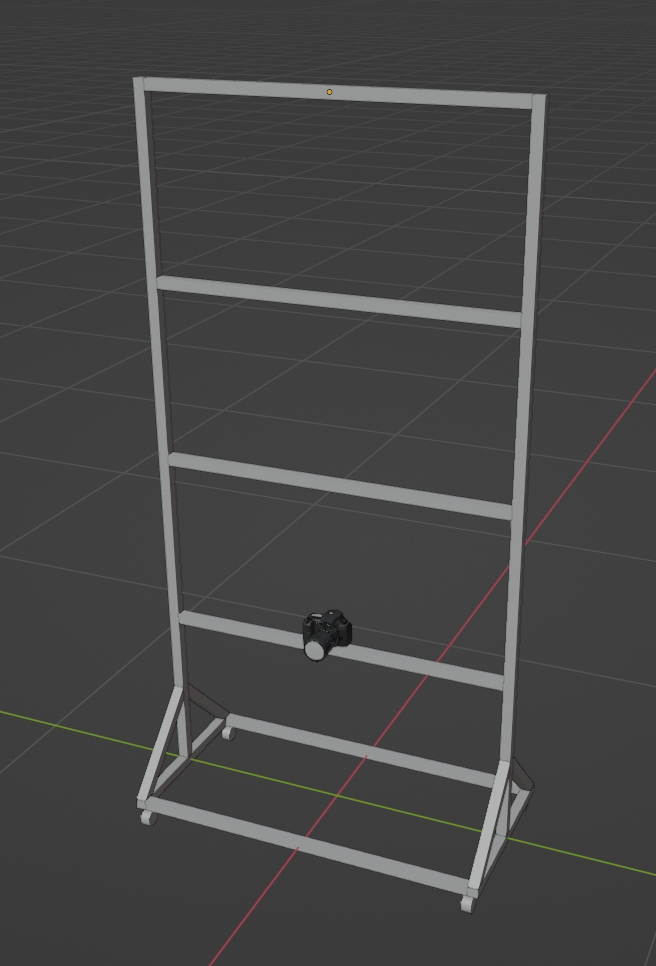
\includegraphics[height=7cm]{figures/frame-design}
    \caption{设计图}
\end{subfigure}
\begin{subfigure}[b]{0.2\textwidth}
    \centering
    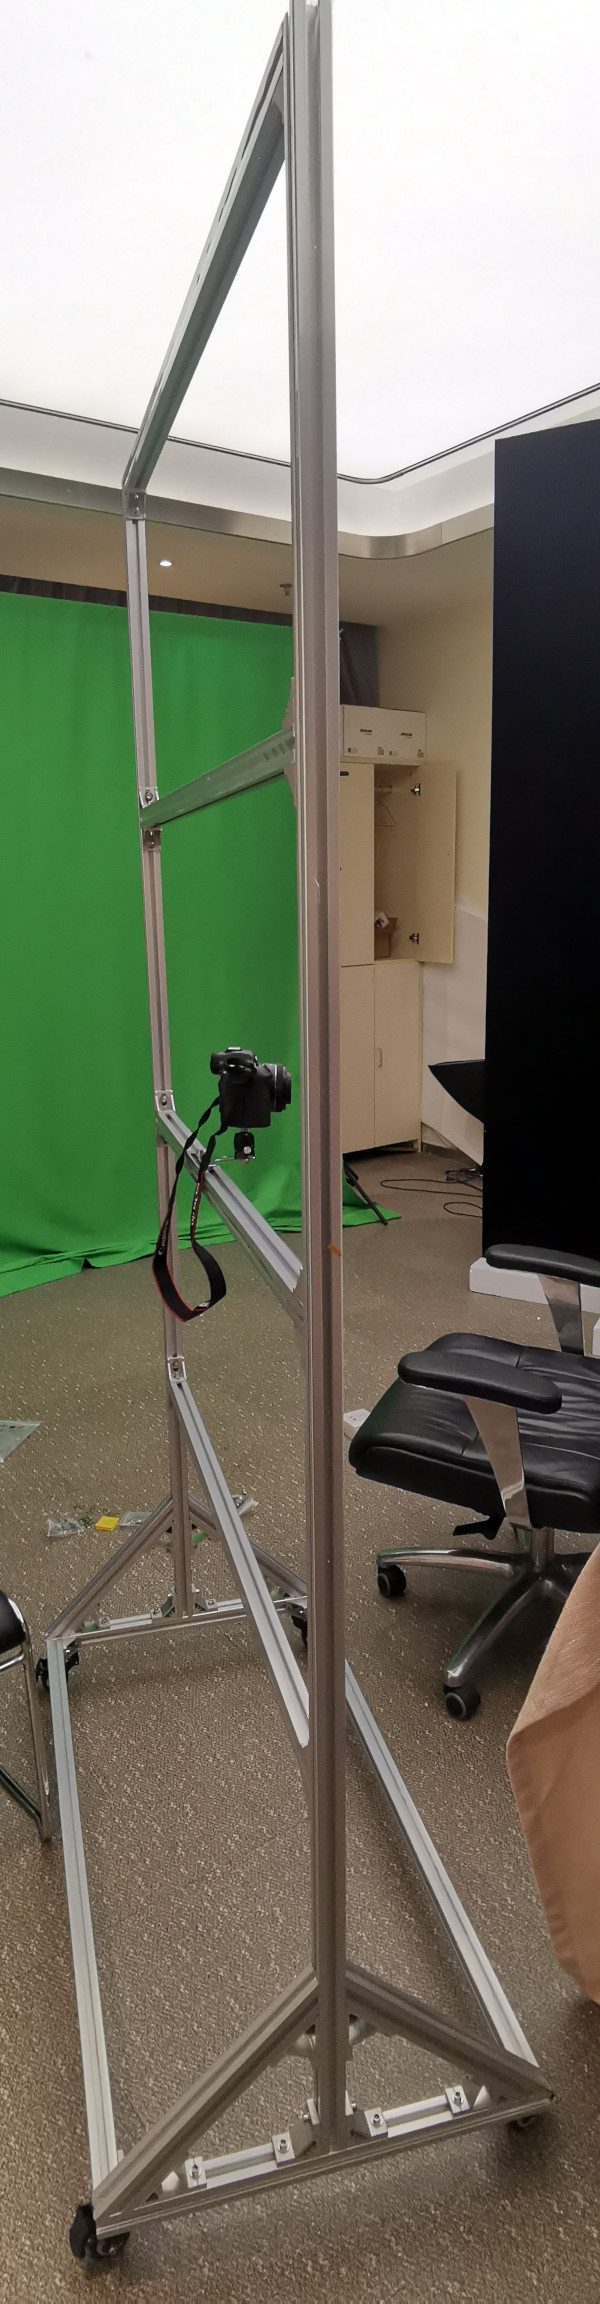
\includegraphics[height=7cm]{figures/frame-impl}
    \caption{组装完成照片}
\end{subfigure}
\begin{subfigure}[b]{0.47\textwidth}
    \centering
    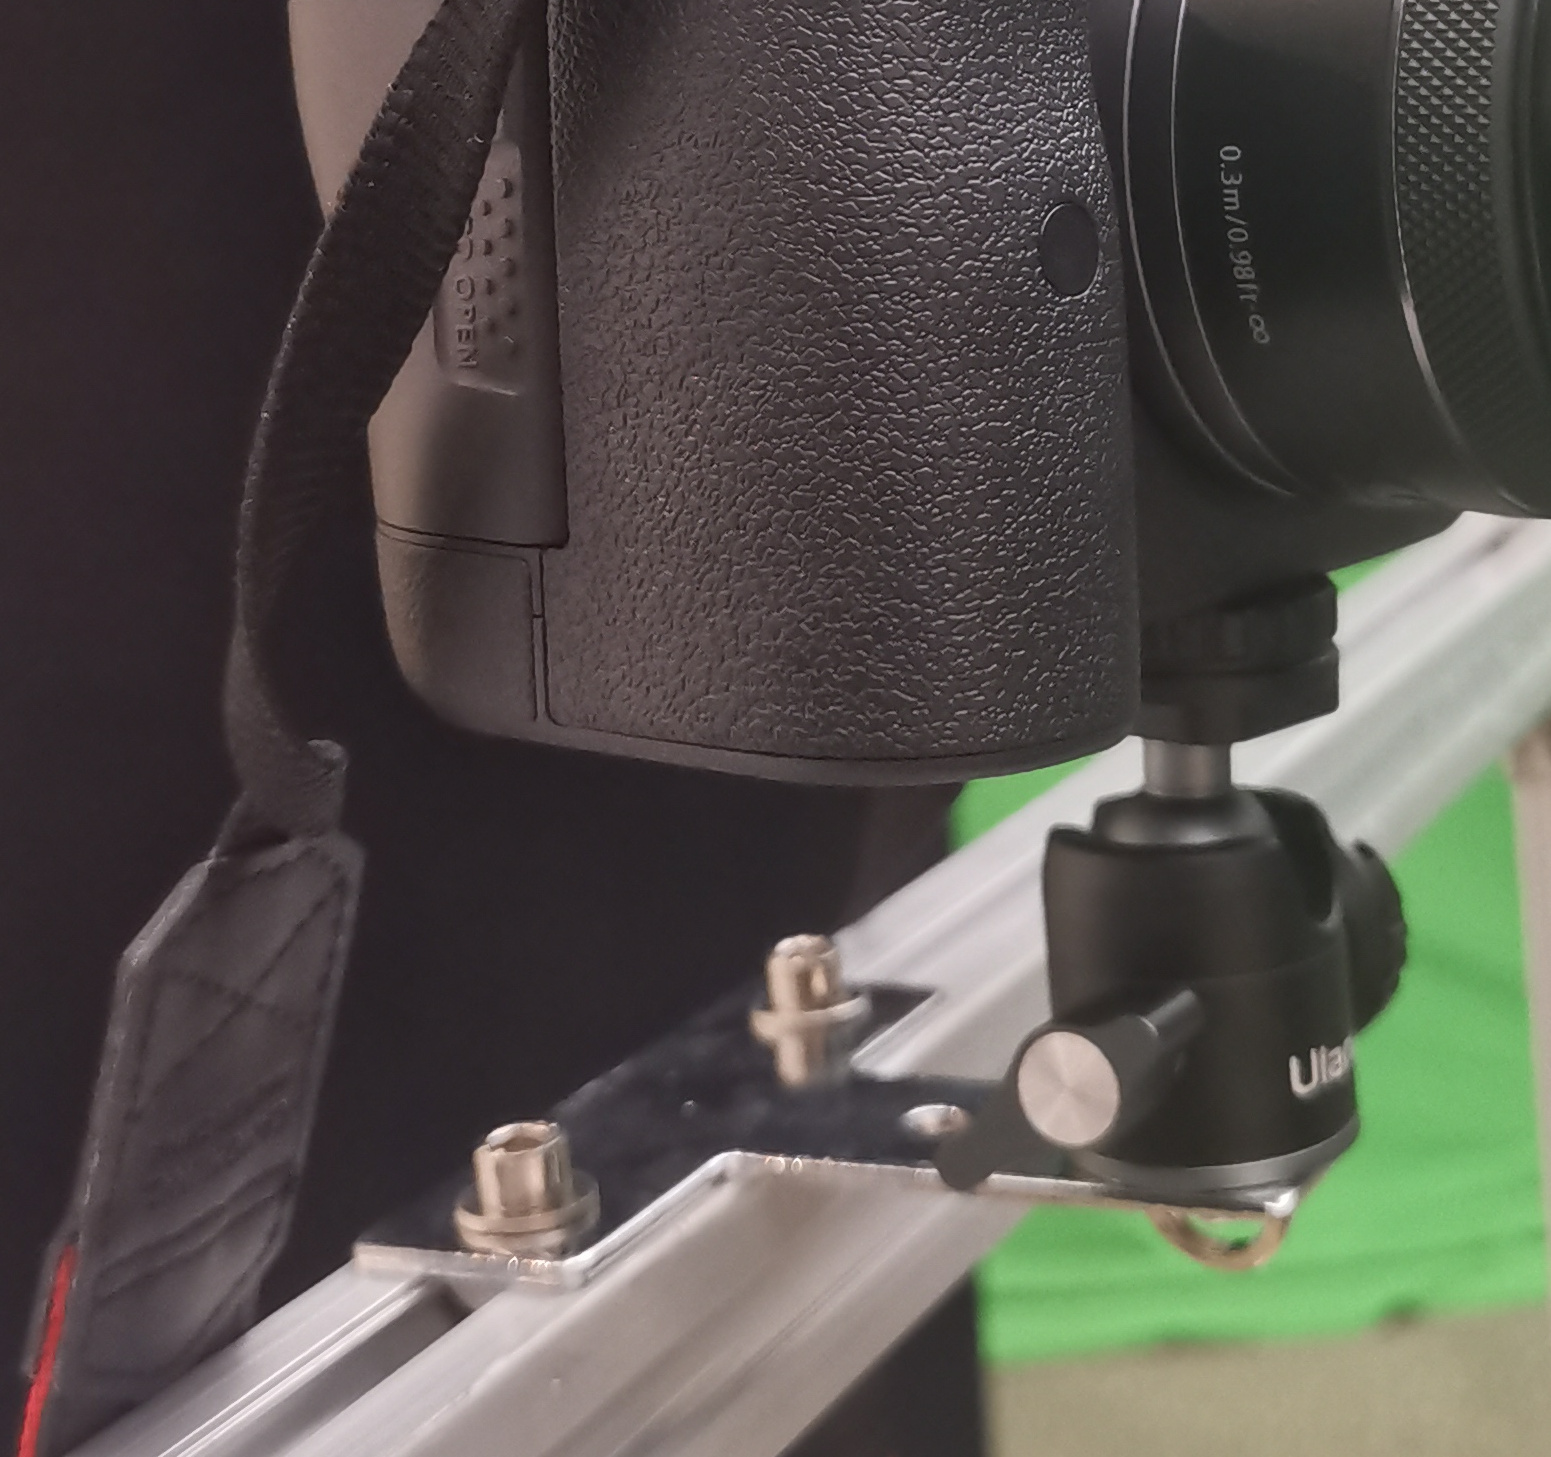
\includegraphics[height=7cm]{figures/frame-camera}
    \caption{相机固定}
\end{subfigure}
\caption{铝型材支架的设计和实现}
\label{fig:frame}
\end{figure}

图\ref{fig:frame}展示了铝型材支架的设计和实现。
单个支架的主体部分由4个2寸脚轮,12.47米3030铝型材以及若干连接件组成。
设计全高2.103米,长1.06米,宽0.53米。
其物料成本约需要700元。
考虑到实验场地可能的变动,支架装配有4个脚轮,方便移动,且这些脚轮带有锁定功能,在使用时也能固定支架的位置。
脚轮固定在矩形底座上,底座则通过大量连接件,尽可能稳固地支撑了两根2米长的竖直铝型材。
在竖杆之间设计有4根长1米的横杆。
每两根间设计间距为0.5米,但得益于本方案使用T型螺母固定,无需打孔,因此这些横杆的位置可根据需要随时调整。

相机可固定在任意竖杆和横杆上的任意位置。
为固定相机,本方案首先将T型连接板通过T型螺母固定在铝型材上,然后将一个球形云台通过1/4英寸螺栓固定在连接板上,最后将相机通过标准的1/4英寸接口固定在云台上。
使用云台可允许相机以三个自由度任意旋转,再加上相机固定位置,横杆位置,以及支架整体的移动,相机最终固定位置的可调节自由度非常高。

总的来说,该支架支撑稳定,使用灵活,完全满足了固定12台相机的需求,为其他部分的实现打下了良好的基础。
同时,通过增加横杆,或增加支架数量的方式,也可以扩展更多相机固定位置。

\section{被动相机同步}
\label{sec:passive_sync}

本方案使用的是CVTE提供的12台消费级微单相机,型号为佳能R6。
将这些相机固定在支架上后,下一步就需要对它们集中进行控制。
其中最简单的形式就是使它们精确地在同一时刻触发快门,以确保后期重建过程不会受到被拍摄对象的位移或形变影响。
为此,本方案中设计了一种用于相机同步的硬件装置。
该装置构造简单,且无须独立供电。它能以很高的时间精度同时触发多台相机的对焦和快门,从而实现人脸多视角数据的捕获。

\paragraph{相机快门触发原理}

为设计该装置,本文首先调查了所使用的相机所有可能的快门触发方式,包括:
\begin{itemize}
\item 相机机身上的快门按钮。该按钮半按可触发对焦,全按可触发快门。
然而使用机械方式触发快门对自动化控制系统来说显然过于复杂,且容易造成不必要的机械震动。
\item 网络接口。该相机支持连接WiFi,并可通过佳能的私有协议或者基于HTTP的Camera Control API控制。
但是无线网络连接会引入毫秒级别的不确定性延迟,因此不适合用于本方案中高精度的同步控制。
\item 快门线接口。该相机支持通过2.5mm快门线接口触发快门,该接口仅需要简单地控制电路通断即可触发对焦和快门。
\item USB连接。该相机支持通过USB连接上游设备,且可通过佳能的私有协议控制。
该方案虽然可以实现更多控制功能,且USB还能直接为相机供电,
但相比上一种方案,上游设备的开发过于复杂,且佳能官方仅提供了Windows平台的SDK,更提高了开发难度。
\end{itemize}
基于这些考虑,本方案最终使用了快门线接口作为相机同步的触发方式。

用于快门线接口的2.5mm插头如图\ref{fig:2.5mm}所示。
该插头的接触部分呈旋转对称的柱体,柱体不同高度上分布有3个独立的接触区域,分别对应对焦控制、快门控制和地线。
其中两根控制线待机时为带有上拉的输入端口,电压为3.3v。当其与地线短接,从而拉至低电平时,即可触发对应的控制。
此外,当手动按下相机快门按钮时,这些控制线也可输出低电平,以控制其他外设。

\begin{figure}
\centering
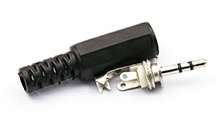
\includegraphics[height=2cm]{figures/2.5mm}
\caption{快门线接口的2.5mm插头}
\label{fig:2.5mm}
\end{figure}

\paragraph{被动同步装置设计}
如上所述,若要控制所有相机同时触发快门,则仅需将所有相机的快门控制线连接到同一个按钮上,在按下该按钮时,使控制线和地线短接即可。
但其中设计的难点在于,被控制的相机数量较多,有12台且可能在未来进一步扩展,且相机在空间上较为分散。
因此,为了节约线材,并提升操作的便捷性和装置的可扩展性,本方案设计了一种可串联的相机控制器。
控制器与控制器,控制器与相机间的连接拓扑如图\ref{fig:passive_sync_topo}所示。
\begin{figure}
\centering
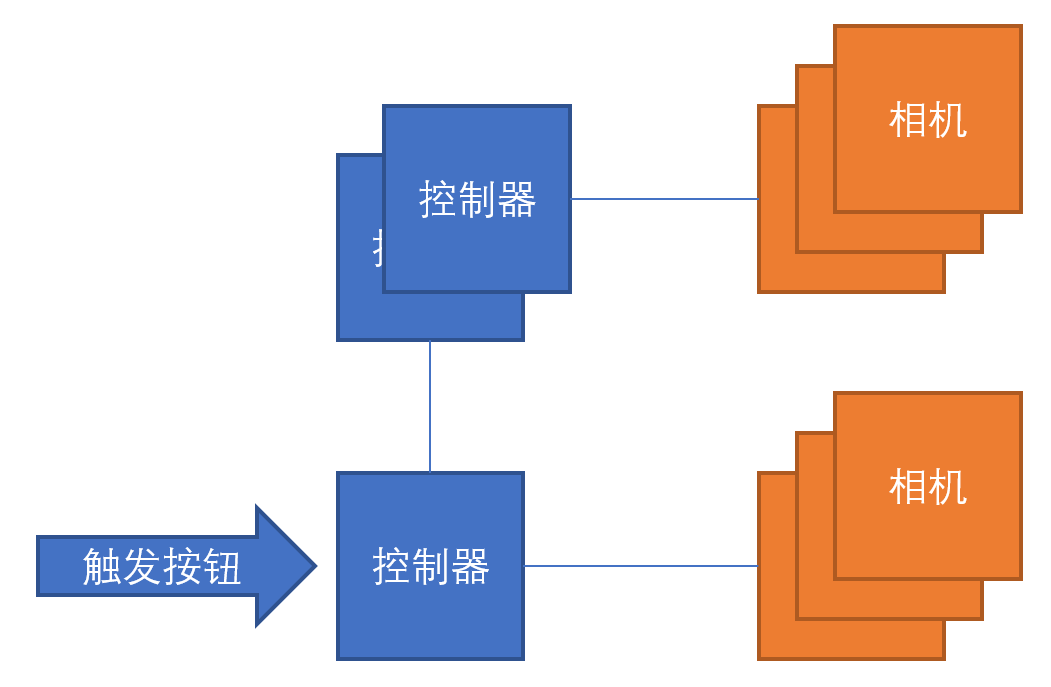
\includegraphics[height=5cm]{figures/passive_sync_topo}
\caption{被动同步装置的拓扑结构}
\label{fig:passive_sync_topo}
\end{figure}
控制器间可以任意方式连接,构成星型、树形或链式等多种不同拓扑,每个控制器最多能与3个其他控制器以及8台相机相连。
该结构可通过增加控制器的方式近乎无限扩展,从而实现对更多相机的控制。
此外,每个控制器上都是对等的,通过任意一个控制器上的按钮均可控制所有相机,提升了系统操作的便捷性。

\begin{figure}
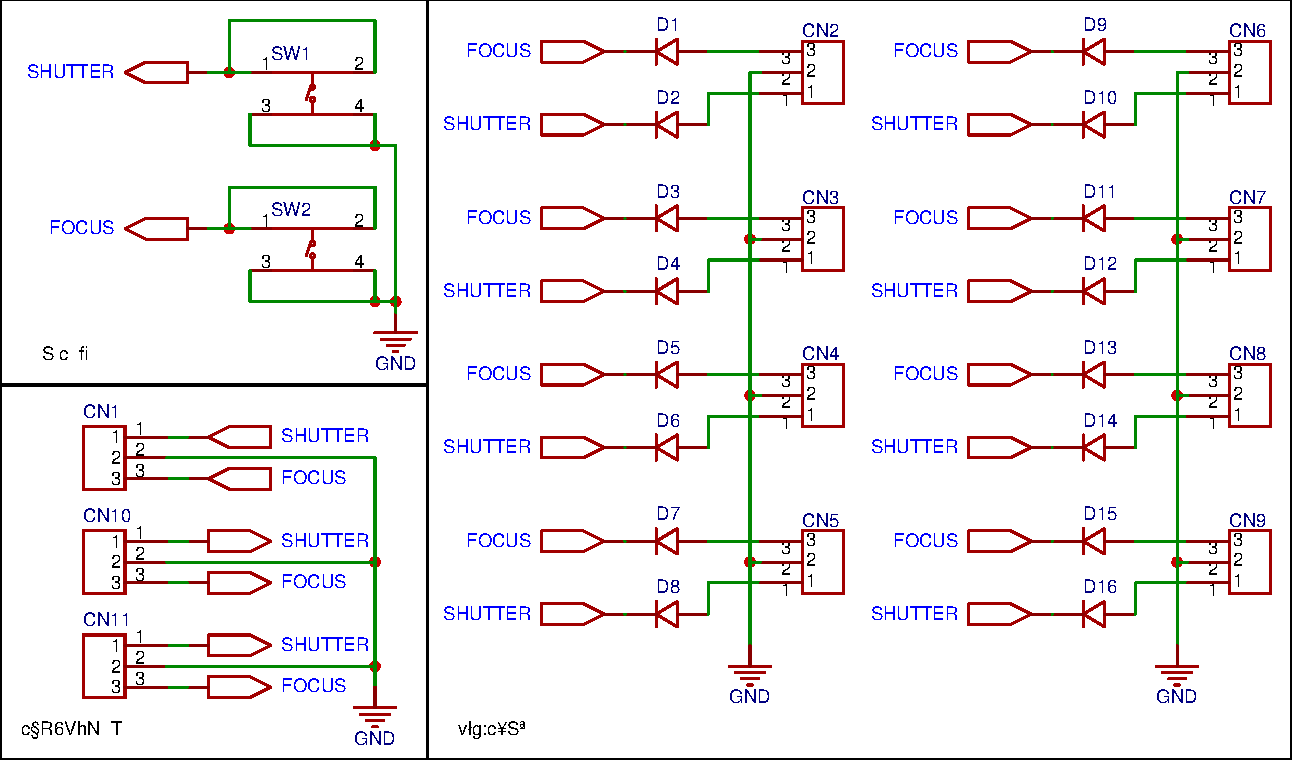
\includegraphics[width=\textwidth]{figures/passive_sync_schematic}
\caption{被动控制器的电路原理图}
\label{fig:passive_sync_schematic}
\end{figure}

\begin{figure}
\centering
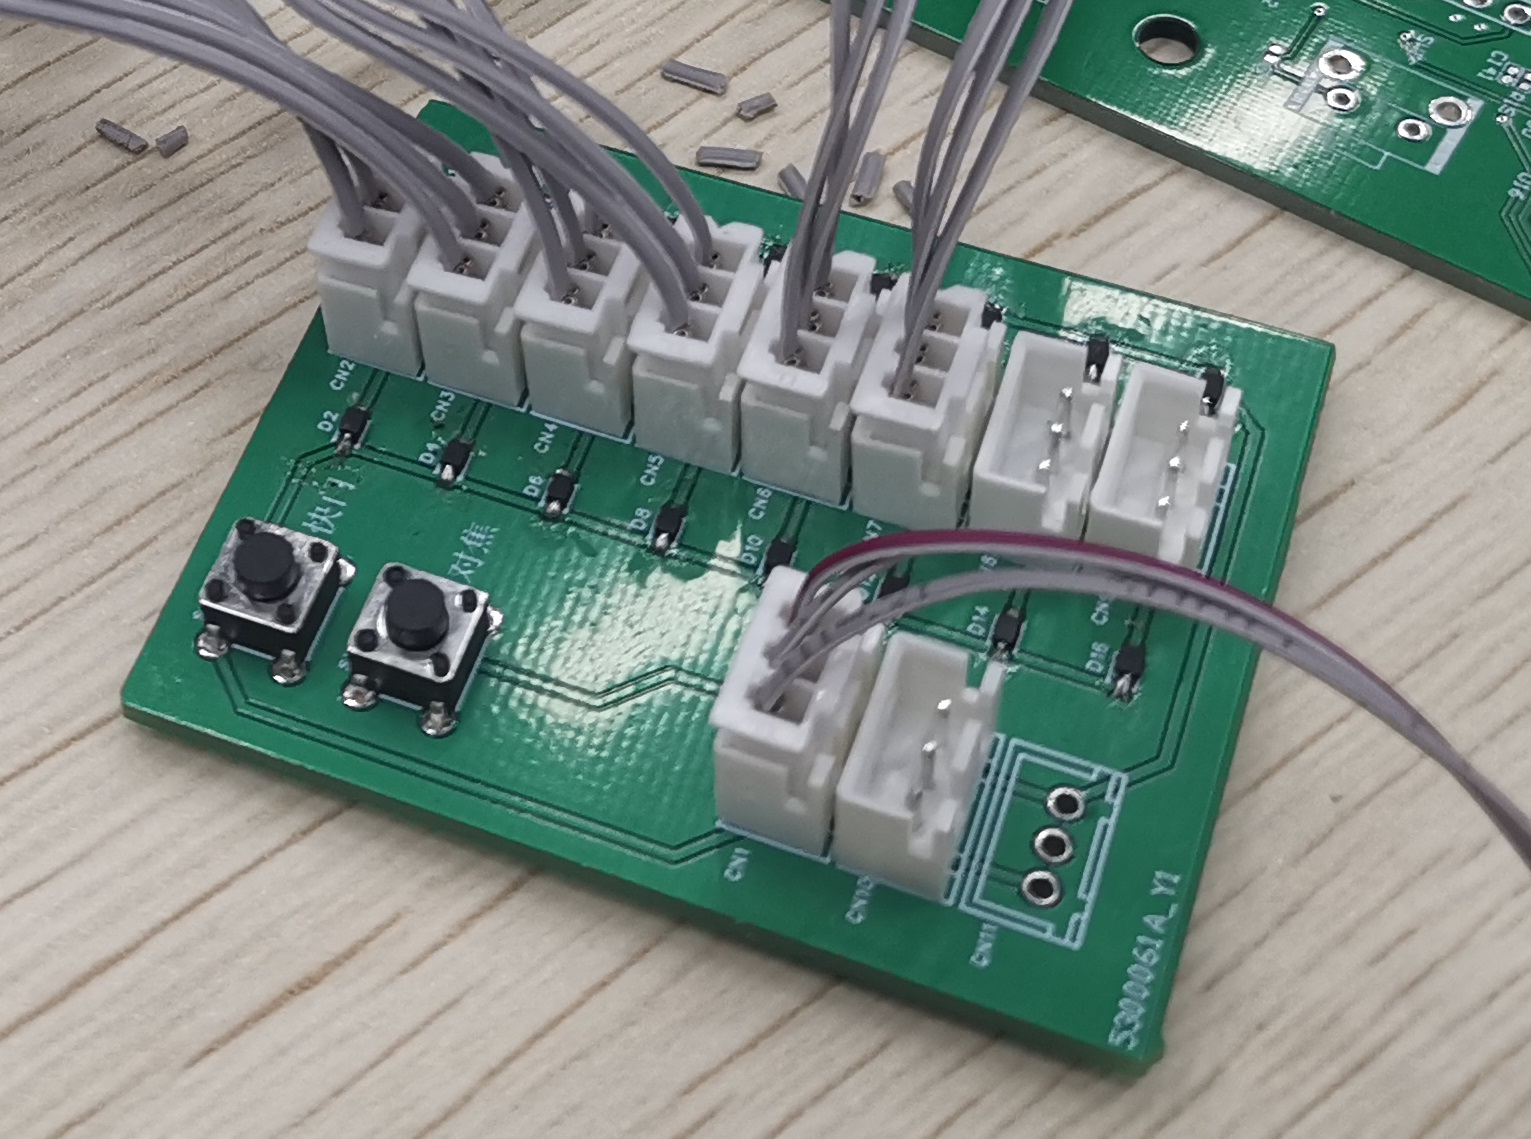
\includegraphics[height=5cm]{figures/passive_sync_controller}
\caption{被动控制器的实物图}
\end{figure}

其中,每个控制器的原理图如图\ref{fig:passive_sync_schematic}所示。
控制器无需供电,它采用机械按钮的形式完成控制线和底线的短接,从而触发相机快门。
控制器之间,以及相机与控制器间均采用AWG28规格的排线连接,
在控制器端均使用了冷压的XH2.54插头;
在相机段则使用了焊接的2.5mm插头。
此外,每个相机接口在连接到总线前均使用了两颗二极管进行隔离,以防止相机间的干扰。
这样可允许在控制器连接时依然可以手动控制单台相机的快门,也能防止在线缆连接时误触发快门。

\paragraph{同步精度测试}

\begin{figure}
\centering
\begin{subfigure}[b]{0.55\textwidth}
    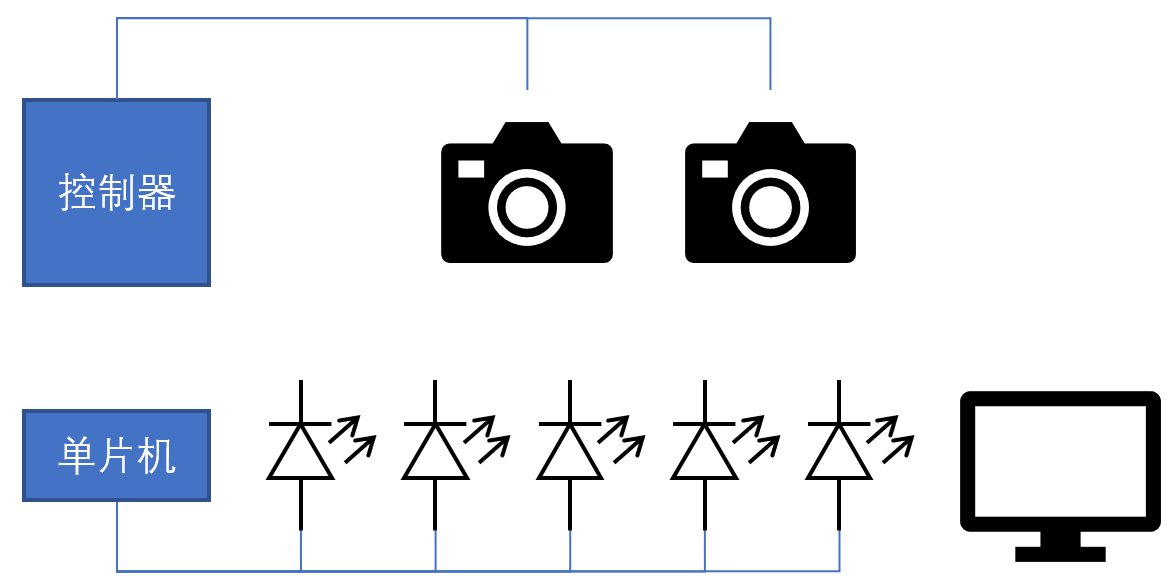
\includegraphics[width=\textwidth]{figures/passive_sync_test}
    \caption{测试过程示意图}
\end{subfigure}%
\begin{subfigure}[b]{0.44\textwidth}
    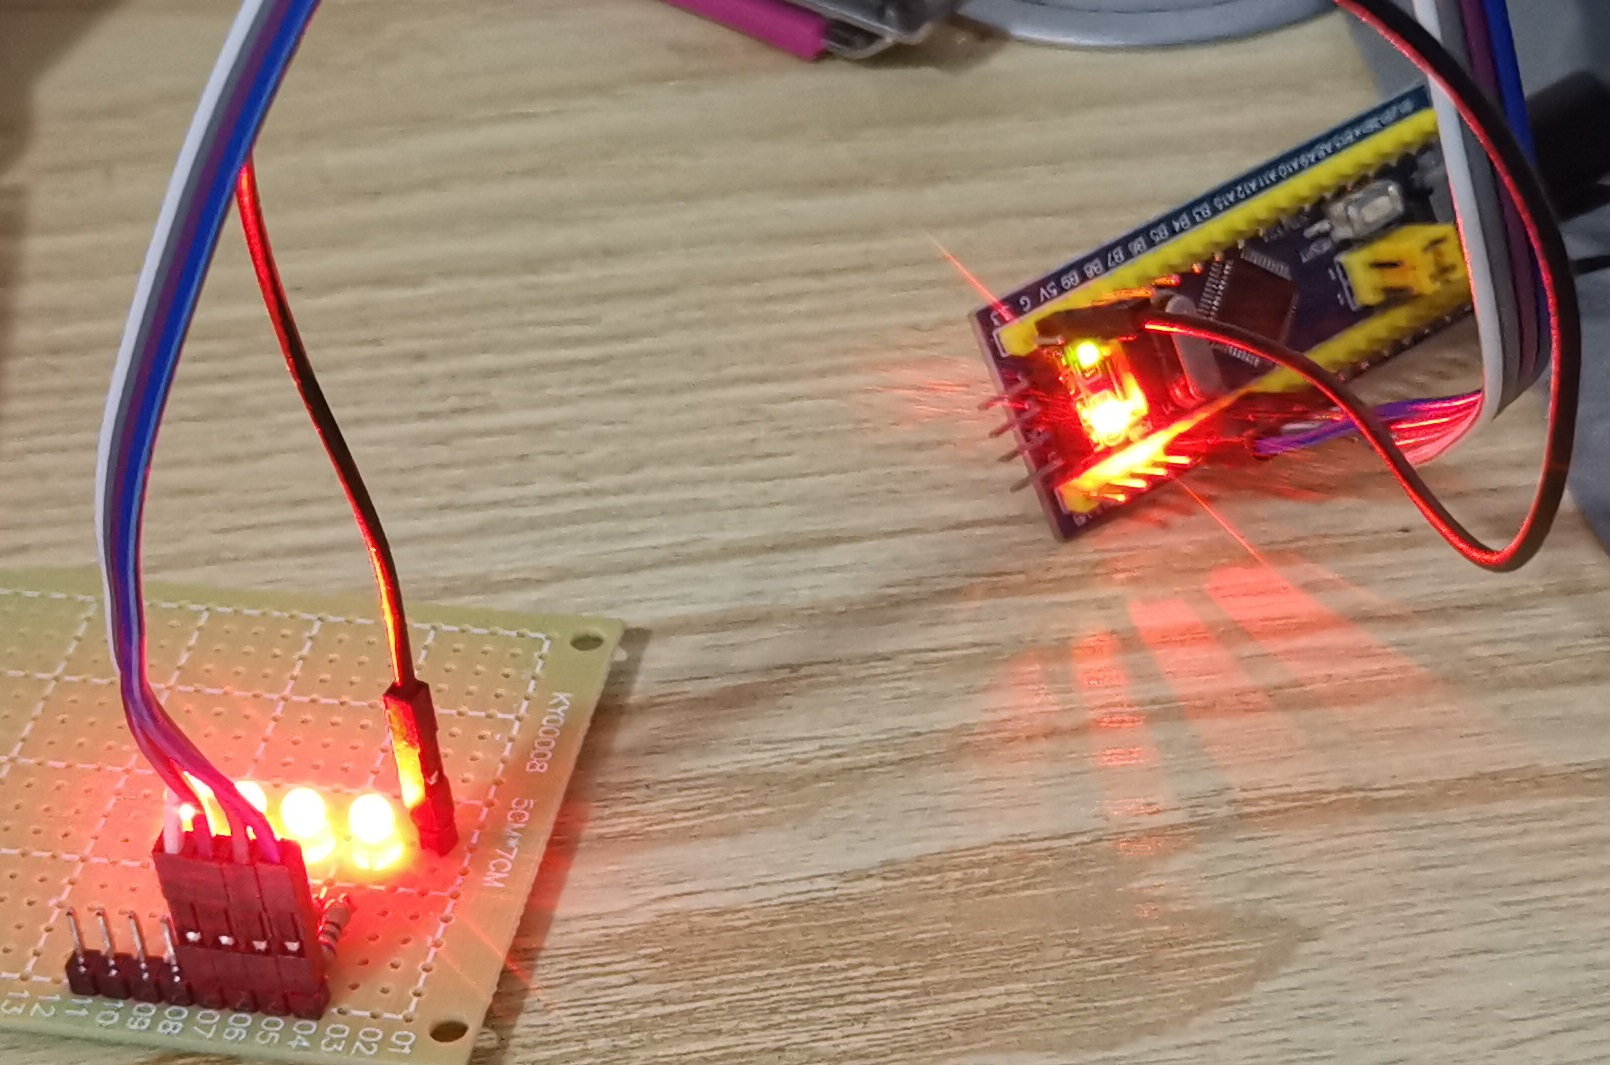
\includegraphics[width=\textwidth]{figures/LED_array}
    \caption{单片机和LED阵列}
\end{subfigure}%
\caption{被动同步装置的同步精度测试装置}
\label{fig:passive_sync_test}
\end{figure}

电场的传播速度非常快,因此,当控制器的按钮被按下时,理论上控制信号能同时送达所有相机。
为了实际测试该装置的效果,本文进行了端到端的同步精度测试。
如图\ref{fig:passive_sync_test}所示,该测试的拍摄目标包括5个由单片机控制的LED灯,以及一个60Hz刷新率的显示器(此处使用iPad)。
其中单片机通过硬件计时器中断精确控制LED灯,每个LED灯的亮灭切换间隔依次为0.5ms、1ms、2ms、4ms、8ms,每16ms这些LED灯的状态完成一次循环。
显示器则显示一个秒表,用于判断16ms以上的时间间隔。

相机拜摆放时,需要使LED灯在不同相机传感器的同一位置成像,以避免滚动快门的影响。
拍摄前,需要将快门速度调整为最快的1/4000秒,以尽量避免相机曝光过程与LED的亮灭切换过程重叠,影响读取LED灯的状态。
测试时,将两台相机连接在控制器上,然后多次使用控制器触发快门。
读取结果时,首先丢弃难以判断LED灯状态的图像,
对剩余图像以二进制编码的形式记录LED灯的状态以及屏幕显示的秒表的时间。
对比同一次快门中不同相机拍摄到的照片中读数即可准确获得两台相机曝光的时间差,即控制器的同步精度。

实验结果显示,多台佳能R6相机间的同步精度小于0.5ms,即每次拍摄中不同相机的读数均相同。该精度已经足够满足实际应用的需求,且已经远高于快门滚动的速度。
因受到相机最高快门速度的限制,未能以更高的精度完成测试。
此外,本文也测试了R6和另一台佳能90D单反相机间同步的精度,结果显示两台相机间有4ms但非常稳定的延迟。

\subsection{多相机内外参联合标定}
\label{sec:camera_calib}

为了准确建模相机成像的光学物理过程,建立三维物体与二维照片之间的对应关系,需要对相机的内参和外参进行标定。
即准确测量采集过程中用到的每一台相机的内参和外参。
其中,内参包括相机的焦距、光心坐标、畸变参数等,
外参则包括不同相机之间的相对位置和姿态。

本方案选用的相机模型是针孔相机模型,这也是在实验中采用的相机所遵循的模型。
由于本实验中相机畸变较小,简单起见,本文选用了OpenCV中默认的径向和切向相机畸变模型\footnote{https://docs.opencv.org/4.7.0/d4/d94/tutorial\_camera\_calibration.html}。
更正式地,假设共有$N$个相机,对于第$i$个相机($i=1,2,\cdots,N$),
内参标定的目标是求解该相机的
焦距$f_x^{(i)},f_y^{(i)}$、
光心坐标$c_x^{(i)},c_y^{(i)}$、
畸变参数$k_1^{(i)},k_2^{(i)},k_3^{(i)},p_1^{(i)},p_2^{(i)}$;
外参标定的目标则是求解该相机在世界坐标系下的
位置$\mathbf{t}^{(i)}=\left(x^{(i)},y^{(i)},z^{(i)}\right)$
和姿态$\mathbf{r}^{(i)}$。
其中$\mathbf{r}\in \mathbb{R}^3$为表示三维旋转群$\mathrm{SO(3)}$的的指数映射向量,
其表示轴为$\mathbf{r}$,角度为$\left\| \mathbf{r}\right\|$的旋转。
世界坐标系的选取是任意的,因此在相机标定阶段,不失一般性地,我们选择第一次快门触发时的标定板坐标系为世界坐标系。
\def\camparam{\delta}
综上,在标定过程中共需要求解$N\times 15$个参数,记为$\camparam$。
在该模型下,对于任意在世界坐标系下的点$\mathbf{X}\in \mathbb{R}^3$,其在第$i$个相机的成像平面的投影点$\mathbf{x}^{(i)}$的计算过程可称为相机投影,记为$\mathbf{x}^{(i)}=\pi(\camparam_i, \mathbf{X})$。

为了解算上述模型中的参数,通常需要使用待标定的相机对一类特殊的物体进行拍摄,称为标定物体。
它们的特点是通常有一些在照片中容易被计算机视觉算法识别的特征点,且这些点容易在不同相机拍摄的照片间进行匹配。
这类物体通常为标定板,即印有棋盘格、二维码、圆形或者其他易于识别的图案的硬质平面板子。
也有一些方法\cite{colmap}使用SIFT等特征点算法来自动从任意被拍摄物体上提取和匹配特征点。但这种方法匹配成功率稍低,且忽略了物体反射光线的各向异性,因此可能会带来一些误差。

\paragraph{数据采集}
\begin{figure}
    \centering
    \begin{minipage}{0.5\textwidth}
        \centering
        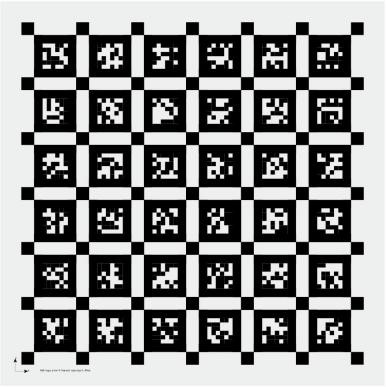
\includegraphics[height=6cm]{figures/april_board}
        \captionof{figure}{April Board上的二维码和棋盘格图案}
        \label{fig:april_board}
    \end{minipage}%
    \begin{minipage}{0.5\textwidth}
        \centering
        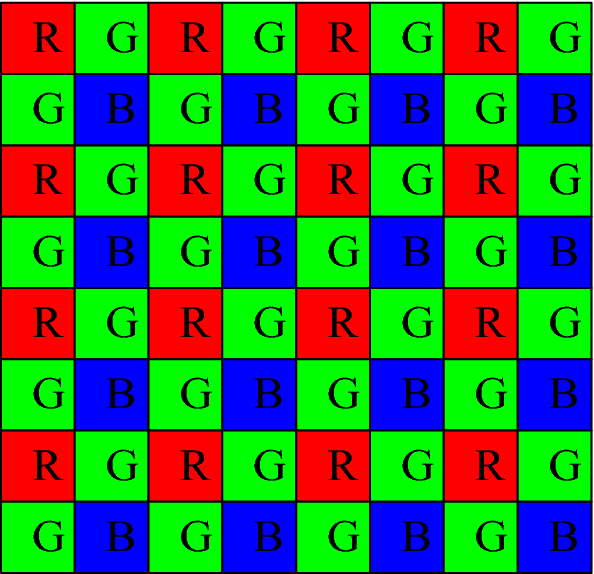
\includegraphics[height=6cm]{figures/bayer}
        \captionof{figure}{Bayer格式照片示意图}
        \label{fig:bayer}
    \end{minipage}%
\end{figure}

本方案中使用的标定物体为April Board,即印有二维码和棋盘格组成的图案的标定板,如图\ref{fig:april_board}所示。
该标定板的尺寸为$800 \times 800$毫米,每个二维码的边长为$88$毫米。
该图案中棋盘格的十字角点可由算法精确完成亚像素级定位,而密集的二维码则便于在不同照片中便捷地匹配角点。
其采用了玻璃基板,以保证标定板的刚性和平整度;
同时采用了氧化铝表面,使标定板表面无明显镜面反射光斑,确保标定板在不同光照条件下的可靠性。

在拍摄标定物体时,需要注意保持相机处于手动对焦模式,关闭光学防抖,以防止其内外参意外发生变化。
并使用前述(第\ref{sec:passive_sync}节)被动相机同步装置同时触发所有相机进行拍摄。转动标定板,重复触发快门15-20次。

\paragraph{相机标定优化目标}
\def\cornerpix{\mathbf{o}}
\def\cornerboard{\mathbf{w}}
本方案中的相机标定算法接收照片中的特征点坐标作为输入,求解上述相机模型中的参数$\camparam$。
正式地,假设共触发了$M$次快门,标定板中共有$K=144$个角点,算法的输入包括第$i$个相机在第$j$次触发快门时拍摄的第$k$个角点($j = 1,2,\cdots,M$、$k = 1,2,\cdots,K$)在像素坐标系中的坐标$\cornerpix_{i,j,k}\in \mathbb{R}^2$;
以及角点在标定板坐标系中的坐标$\cornerboard_k\in \mathbb{R}^3$。
由于每次触发快门时标定板都由人工转动,因此其在世界坐标系中的位置也是未知的,故将第$j$次快门时标定板坐标系到世界坐标系的刚体变换$T_{j}(\cdot)\in \mathrm{SE(3)}$也做为未知量。
其中固定$T_{1}$为幺元,即$T_{1}(X) = X$,以确定世界坐标系的位置。
则本文中的相机标定问题可以表示为以下最小二乘优化问题:
\begin{equation}
    \label{eq:calib_opt}
    \argmin_{\camparam,T} \sum_{i,j,k} \left\| \cornerpix_{i,j,k} - \pi\left(\camparam_i, T_j(\cornerboard_k)\right) \right\|_2^2
    \text{。}
\end{equation}
为实现该目标,首先需要在每张照片中识别角点,并以亚像素级精度精确定位其坐标$\cornerpix_{i,j,k}$。
本节后续将介绍角点的识别、精确定位,模型初始化及上述优化问题的具体求解方法。

\paragraph{角点识别}为识别标定板中可供拟合的角点,本文首先识别照片中的二维码,并将二维码的四个角作为角点的候选点。
本文所用标定板上的二维码为AprilTag,本文实现的识别算法也是基于其开源的方法\cite{AprilTag}。
该算法是一个自下而上的算法,它首先从照片中识别直线段,然后将直线段组合成四边形,最后试图将四边形区域识别为二维码。得益于二维码的纠错功能,虽然该方法召回率稍低,但查准率非常高。同时二维码中存储的信息可用于角点在不同照片中的匹配。

本文所实现的版本的输入为相机拍摄的,原始Bayer格式的照片,该照片是单通道图像,其中RGB像素排列如图\ref{fig:bayer}所示,每$2\times 2$个像素中包括一个红色像素、两个绿色像素和一个蓝色像素。每种像素的传感器前带有滤光片,仅允许特定波长的光被传感器捕获。因此,Bayer格式的照片中,每个像素的值即为该像素对应的颜色通道的光照强度。
为了减少冗余的数据处理流程,并保持全流程的可解释性以准确控制误差,本方案直接使用了原始照片,而没有使用常见的相机后处理后输出的RGB格式图像。

由于我们所拍摄的照片分辨率远超二维码识别所需,因此本文先对照片进行降采样。
其具体方法是,首先在每4个像素中仅取一个绿色像素,以排除颜色对二维码识别的影响;
再进行5倍平均池化,即最终降采样后的图像长宽为原图的$1/10$。
以此降低算法耗时并大大降低照片中的噪声等级,提升算法的鲁棒性。
在低分辨率的图像上完成二维码识别后,二维码的四个角的坐标将被重新映射回完整分辨率的像素坐标,以初始化后续的精确定位步骤。

% 本文使用的相机拍摄的原始照片分辨率高,可达$5472\times 3648$;
% 且宽容度高,其量化后的亮度可达约13000级,相比普通JPG照片仅有256级。
% 因此,本文在\cite{AprilTag}的基础上,设计了尺度、亮度无关的直线段识别算法,使其更加鲁棒,并减少算法超参数调节的麻烦。
% \TODO{尺度、亮度无关的直线段识别算法}

\paragraph{角点精确定位}在上一步识别出角点后,该步骤依据角点周围的像素值,获取这些角点尽可能精确的像素坐标$\cornerpix_{i,j,k}$,以保证标定的精度。
该步骤的难点在于,算法需要对失焦造成的模糊、成像过程中的噪声等因素足够鲁棒,并达到亚像素级的精度。
本文采用的算法为\citet{ROCHADE}提出的精确角点定位算法,其基本思想为:
使用一个二维多项式函数对角点周围的像素进行拟合,然后以该多项式函数的鞍点作为该角点的精确像素坐标。

具体地,本文首先需要从照片原始数据获取单通道灰度图。
该灰度图在标定板区域的每个像素值应表征标定板表面反射的总光强,而不与颜色有关。
为此,需要对红色、蓝色像素值进行缩放,使其与绿色像素匹配(相当于相机的白平衡操作),其缩放系数与环境光照、标定板材质等有关。
本文假设标定板任意位置反射的光线的波长分布是均匀的。
因此,本文首先对上一步求得的二维码区域求凸包,以定位照片中的标定板,并调整缩放系数以使该区域中不同颜色像素的均值相等。
然后,对该图使用半径为$r$的圆锥形kernel进行滤波,以使像素值平滑,从而能更好地被多项式函数拟合。
最后,以角点的当前估计位置为中心,使用二阶二维多项式函数对周围的$2r+1 \times 2r+1$个像素进行最小二乘拟合:
\begin{equation}
    \label{eq:poly}
    \hat{a} = \argmin_{a} \sum_{x,y} \left(\bar{I}(x, y) - (a_0 x^2 + a_1 y^2 + a_2 xy + a_3 x + a_4 y + a_5)\right)^2\text{。}
\end{equation}
在实现上,本方案直接使用解析公式求解该线性最小二乘问题。并求该二维多项式函数的鞍点作为该角点新的估计位置:
\begin{equation}
    \label{eq:subpixel}
    \begin{cases}
        x' &= -\dfrac{\hat{a}_2 \hat{a}_4 - 2 \hat{a}_1 \hat{a}_3}{\Delta} \\
        y' &= -\dfrac{\hat{a}_2 \hat{a}_3 - 2 \hat{a}_0 \hat{a}_4}{\Delta}
    \end{cases},\quad
    \Delta = 4 \hat{a}_0 \hat{a}_1 - \hat{a}_2^2
    \text{,}
\end{equation}
并如此迭代,直到角点的估计位置收敛,该收敛的位置即为$\cornerpix$。
在此过程中,若估计位置超出了图像范围,或$\Delta < 0$,则将该角点排除。
$\Delta < 0$的原因通常是该角点被其他物体遮挡,或者受到其他物体投下的阴影影响。

\def\cornerincode{\hat{\cornerpix}}
在该算法中,$r$的选取可能对结果产生较大影响。较大的$r$将能利用照片中更多像素的信息,从而对噪声更加鲁棒,但也不能过大,否则周边的二维码,或相邻的其他角点等无关信息将影响拟合结果。为此,本文依据上一步识别到的二维码的尺寸以自适应地选择$r$。令$\cornerincode_{i,j}$为照片中第$i$个二维码的第$j$个角点的估计位置,$j\in\{0,1,2,3\}$,以顺时针方向排列,则$r$的选取为:
\begin{equation}
    \label{eq:r}
    \begin{aligned}
        l_{i,\textrm{edge}} & = \min_j\left(\|\cornerincode_{i,j} - \cornerincode_{i,j+1\bmod 4}\|\right)\text{,} \\
        l_{i,\textrm{diag}} & = \min\left(\|\cornerincode_{i,0} - \cornerincode_{i,2}\|, \|\cornerincode_{i,1} - \cornerincode_{i,3}\|\right)\text{,} \\
        r & = \min_i\left\{0.07 l_{i,\textrm{edge}}, 0.05 l_{i,\textrm{diag}}\right\}\text{。}
    \end{aligned}
\end{equation}

\paragraph{多相机内参标定与外参传递}
在第一阶段,本文将对每台相机分别进行标定,获得各相机的内参初始化值
并估计标定版在每次触发快门时与各台相机的相对位置。
具体地,本文依据相机和镜头厂商提供的传感器尺寸、图像分辨率、镜头焦距初始化相机内参$f$、$c$。
然后调用OpenCV中单台相机标定的算法,使用PnP算法求解标定板在每次触发快门时与相机的相对位置$T_{i,j}$;
并使用Levenberg-Marquardt算法对这些参数进行调整。

由于不同相机的同一次快门的触发是严格同步的,因此可以认为若不同相机在同一次快门的触发时,拍摄到的标定板在世界坐标系中的位置是相同的。
据此可将每台相机,以及每次快门触发作为节点,构建二部图,图中的边表示该相机在该次快门中拍摄到了标定板。
若该二部图是连通图,则可迭代地将所有相机、所有快门触发中的标定板的位置传递到世界坐标系中,
如算法\ref{alg:calib_init}所示。
并最终获得$\delta$和$T$中所有参数的初始化值。

\begin{algorithm}[t]
    \caption{外参传递}
    \label{alg:calib_init}
    \begin{algorithmic}[1]
        \Require 连通二部图$(V,E)$;第$j$次快门时标定版坐标系到相机$i$坐标系的刚体变换$\hat{T}_{i,j}\in SE(3),(i,j)\in E$
        \Procedure{外参传递}{$V,E,\hat{T}_{i,j}$}
            \State $C \gets \emptyset$\Comment{已传递的相机集合}
            \State $T_{1} \gets \mathbf{I}$\Comment{以第$1$次快门时标定版坐标系作为世界坐标系}
            \State $S \gets \{1\}$\Comment{已传递的快门触发集合}

            \While{$C \cup S \neq V$}
                \State $i \gets \forall i\in V| i\notin C, \exists j\in S| (i,j)\in E$
                    \Comment{选择与已知位置的标定板相邻的相机}
                \State $U_{i} \gets T_{j}\hat{T}_{i,j}^{-1}$
                    \Comment{相机$i$到世界坐标系的变换}
                \State $C \gets C \cup \{i\}$
                \ForAll{$j | (i,j)\in E, j\notin S$}
                    \State $T_{j} \gets U_{i}\hat{T}_{i,j}$
                        \Comment{第$j$次快门时标定版到世界坐标系的变换}
                \EndFor
                \State $S \gets S \cup \{j\in V| (i,j)\in E\}$
            \EndWhile
            \State \Return $U, T$
        \EndProcedure
    \end{algorithmic}
\end{algorithm}

\paragraph{集束调整}在第二阶段,本文将对所有相机进行集束调整,即直接使用公式\eqref{eq:calib_opt}中的目标函数,在上一阶段的初始化值的基础上,同时优化模型中的所有参数。
具体地,本文使用了Levenberg-Marquardt算法\cite{lm},对目标函数进行优化求解。
并手动实现了公式\eqref{eq:calib_opt}的雅克比矩阵的解析求解算法,以提升算法的速度和收敛精度。

然后,排除掉误差较大的角点,再次重复上述优化过程,并如此迭代数次,每次使用更严格的误差阈值进行排除。
这些误差较大的角点通常是由于角点定位不准确造成的,因此,将其排除后可以提高标定的精度。
该优化过程最终得到的相机参数$\camparam$即为所求的最终的相机标定结果。


\section{基于反射球的光源标定和HDRI合成}

除了相机外,在实验室中拍摄,环境光照信息也可以提前采集,从而获得比用算法从人脸照片中估计更精准的结果。
这些信息可用于后续逆渲染的优化之中。
如前文所述,本装置使用的照明为4盏带有柔光箱的摄影灯,均布置在被拍摄对象正面180°的范围内。光源标定的目的是获取被拍摄对象所处的空间中的每个位置上来自每个方向的光照强度,即光场信息。
但本设备的柔光箱据被拍摄对象约1.5米远,相比来说,人脸的尺度较小,因此,本文假设所有光线均来自无限远,即该光场的分布近似于与空间位置无关而只与光线入射方向有关。

光照强度和方向的对应关系可被编码在一张HDRI图像(High Dynamic Range Image,高动态范围图像)中,该图像中的每个像素点对应于一个方向,像素点的颜色值则对应于该方向上的光照强度和频率分布。
其与普通的照片保存格式不同,之所以称之为是高动态范围,是因为其每个像素点的颜色值通常作为浮点数保存,因此可以同时记录很强和很弱的光照,同时保持较高的精度。
使用该技术编码的光照信息也常被用于计算机图形学领域。
如图\ref{fig:HDRI}是一张以本节所述方法合成的,记录了本文目前实验环境的HDRI图像。
\begin{figure}
\centering
\TODO{HDRI图像}
% 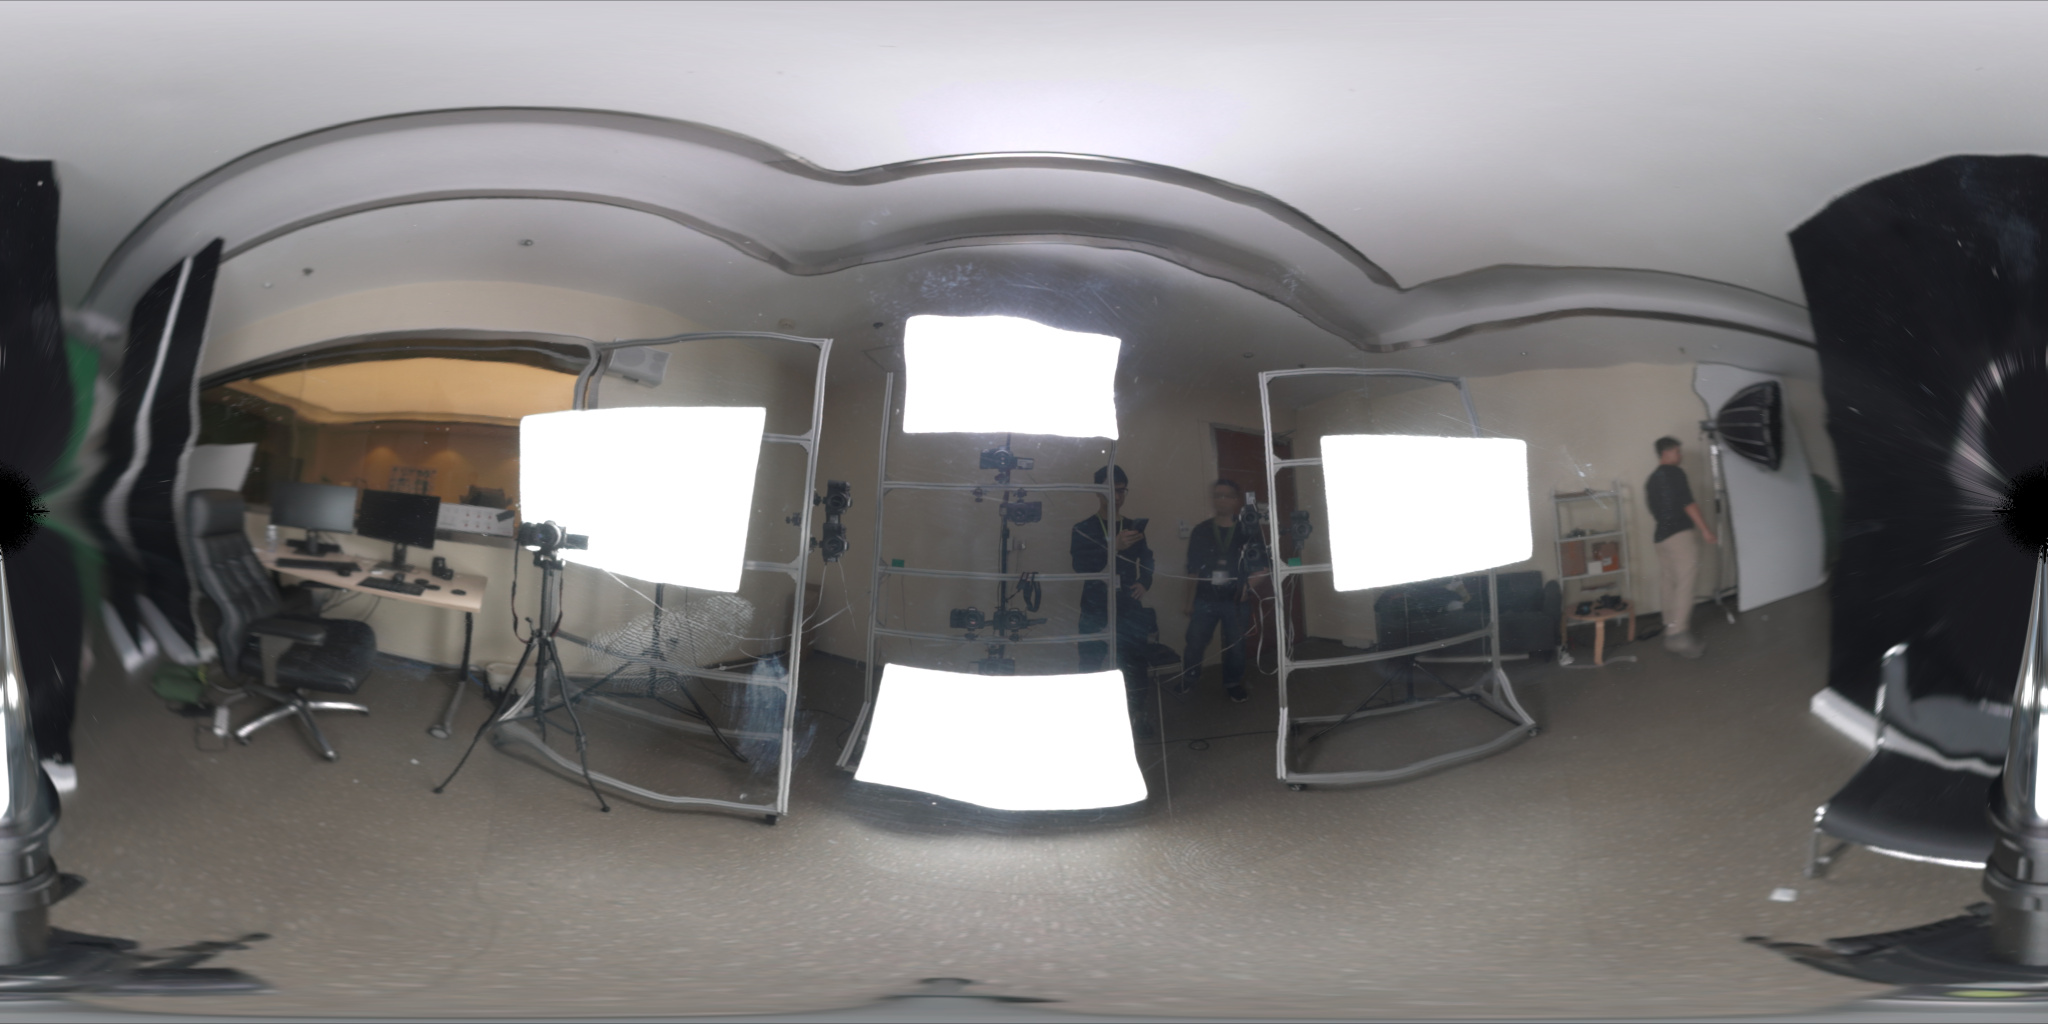
\includegraphics[width=\textwidth]{figures/HDRI}
\caption{实验环境全景HDRI图像}
\label{fig:HDRI}
\end{figure}

\paragraph{数据采集}
为了收集用于合成HDRI的数据,本文将一个全镜面金属的反射球放置于原被拍摄对象头部的位置,然后通过WiFi控制一台靠近中心的相机,继续固定对焦和光圈设置,改变其快门速度和ISO,以捕获该球不同曝光的照片。
通常拍摄的相邻两张照片亮度相差约一倍,共拍摄约8张照片。
这是因为相机的传感器所能记录的最大光照强度是有限的,而若只使用更低的曝光,则由于信噪比的下降,导致最终合成的HDRI中的噪声更多。
使用多种不同的曝光参数拍摄即可同时保留亮部和暗部的细节。
后续步骤将直接使用原始Bayer格式的照片,尽可能保留其中信息,同时获取准确的噪声等级估计。

\paragraph{HDRI合成}
该步骤的目的是将上述拍摄的多张照片中各自最可靠的部分(信噪比高,且未超出传感器量程范围)融合为一张HDRI。
为此,本文设计了一种类似卡尔曼滤波的融合算法。
其基本思想是:将不同照片中的同一像素点的读数视为对同一光照强度的不同测量值,并有不同的测量噪声方差,据此对多个观测值加权平均,得到最可能接近真值的估计值。

本方案使用的相机的传感器中包含了约50万个完全不接受入射光线的像素,这些像素可用于估计黑场(即完全无入射光线时传感器的读数)和测量噪声的方差。
由于数据量非常充裕,这里对每张照片和每个通道分别进行了估计。
计照片$i$中通道$c\in\{\mathrm{r},\mathrm{g1},\mathrm{g2},\mathrm{b}\}$的黑场为$b_{i,c}$,方差为$\sigma_{i,c}^2$。
然后,根据拍摄参数计算每张照片的相对亮度,该值与拍摄的曝光时间和ISO设置成正比。
并将照片据此由暗到亮排序为$\mathcal{I}^{(1)}, \mathcal{I}^{(2)}, \cdots, \mathcal{I}^{(n)}$。
由于原始照片中记录的传感器读数和实际光照强度呈很好的线性关系,
因此可根据读数在每两张相邻照片间通过最小二乘法计算其准确的相对亮度比例:
\begin{equation}
r_i^* = \argmin_{r_i} \sum_{j|\mathcal{I}^{(i+1)}_j < \xi} \left[r_i (\mathcal{I}^{(i)}_j - b_{i,c}) - (\mathcal{I}^{(i+1)}_j - b_{i+1,c})\right]^2
\text{,}
\end{equation}
其中$\xi$为使用ExifTool读取的“线性上界”(Linearity Upper Margin),$j$为像素索引。
该问题为线性最小二乘,可直接求其解析解。
该比例理论上应与之前从拍摄参数计算的值相同,但实际可能由于相机校准误差或其他原因而有所偏差。
\begin{figure}
\centering
\import{build/figures}{HDRI_stats.pgf}
\caption[HDRI输入照片读数统计]{HDRI输入照片读数统计。
(a)展示了相邻曝光的两张照片中同一位置的像素值之间的对应关系,其背景的直方图表示较暗照片像素数量在不同像素值上的分布。
可见在超出量程前它们具有很好的线性关系,但通过曝光时间估计的亮度比例与实际有明显偏差。
(b)展示了观测噪音与ISO设定间的关系。}
\label{fig:HDRI_stat}
\end{figure}
如图\ref{fig:HDRI_stat}a展示了其中一对照片的读数对应关系,可见实际拟合的比例与从拍摄参数计算的有明显偏差。
最后根据这些相对值$r_i^*$,令任意照片的亮度系数为$1$,可求得所有照片的亮度系数$e_i$。

有趣的是,虽然理论上ISO越高则噪声水平将越高,但本方案使用的相机在ISO从200增加至400时噪声水平却无明显上升,反而是黑场由512上升到了2048。由此可以推测或许相机在这两种不同配置时处于不同的工作模式。

在获得了这些参数后,假设观测噪声服从高斯分布,即可从暗到亮递推地合成HDRI。合成的过程可表示为:
\begin{equation}
\begin{aligned}
    \mathcal{J}^{(1)} &= e_1 \left(\mathcal{I}^{(1)} - b_{1,c}\right),\quad
    \hat{\sigma}_{1,c}^2 = e_1^2 \sigma_{1,c}^2 \\
    \mathcal{J}^{(i)}_j &= \begin{cases}
    \frac{e_i^2 \sigma_{i,c}^2 \mathcal{J}^{(i-1)}_j + \hat{\sigma}_{i-1,c}^2 e_i \left(\mathcal{I}^{(i)}_j - b_{i,c}\right)}{\hat{\sigma}_{i-1,c}^2 + e_i^2 \sigma_{i,c}^2} & \text{if } \mathcal{I}^{(i)}_j < \xi \\
    \mathcal{J}^{(i-1)}_j & \text{otherwise}
    \end{cases}\\
    \hat{\sigma}_{i,c}^2 &= \frac{e_i^2 \hat{\sigma}_{i-1,c}^2 \sigma_{i,c}^2}{\hat{\sigma}_{i-1,c}^2 + e_i^2 \sigma_{i,c}^2}
    \quad (i > 1)\text{,}
\end{aligned}
\end{equation}
其中$\mathcal{J}$为每步合成的照片,$\mathcal{J}^{(n)}$即为最终所需的HDRI。
该递推过程与卡尔曼滤波中的融合新的观测值的过程类似,且可以由贝叶斯公式导出,即通过以$\mathcal{J}^{(i-1)}$为均值的先验分布,融合以$e_i\left(\mathcal{I}^{(i)} - b_{i,c}\right)$为均值的观测,推导以$\mathcal{J}^{(i)}$为均值的后验分布。

该融合过程具有以下理想的性质:
较暗的照片信噪比较高,其由于具有较大的$e_i$而在合成时方差较大,从而权重更低;
照片中超出传感器量程($\geq\xi$)的部分则完全不会影响合成结果;
ISO较高的照片由于噪声方差较大(如图\ref{fig:HDRI_stat}b),也能自动在合成中降低权重。

\paragraph{像素重映射}

\section{主动相机/闪光灯同步}

主动相机同步装置有单片机等实时控制系统控制,能独立控制每台相机、闪光灯触发延迟,最多24个通道。可用于快速抓拍不同闪光灯照明下的照片

\paragraph{主动同步装置硬件设计}

\paragraph{主动同步装置软件设计}

\paragraph{滚动快门原理}

\paragraph{闪光灯触发延迟快速标定方法}

\section{照片拍摄和整理流程}

\paragraph{同步装置连接与设定}

\paragraph{拍摄采集对象}

\paragraph{相机、光源标定数据采集}

\paragraph{照片拷贝和整理}

\section{初步验证}

作为该实验平台实用性的初步验证,本文利用该平台采集的数据使用传统的计算机视觉方法尝试重建人脸模型。

本文首先使用Colmap完成人脸的稀疏以及稠密点云重建。\TODO{参数调整}

然后,本文使用FlameFitting工具,将FLAME 3D模型配准到稠密点云上,得到初步的人脸几何形状。

然而,该配准的效果并不理想。因此本文使用Blender同时导入点云和几何形状,并手动调整模型顶点位置以完成更精确的配准。

最后,本文通过Unwrap方法,将照片映射到UV空间,每个视角获得一张纹理贴图,再将这些纹理贴图通过以下方式进行融合,最终获得一个带纹理的3D人脸模型。

\TODO{融合方式公式}

\TODO{结果图}

\section{后续工作}

然而,这种方法仅仅是对该平台采集的数据的初步利用,仅发挥了该平台的一小部分价值。
该平台的设计目标是用于运行可微分渲染算法,后续的研究者们将能利用该平台开展诸多基于可微分渲染的研究,例如:
\begin{itemize}
\item 在传统计算机视觉重建的几何形状的基础上,利用可微分渲染算法,实现符合基于物理的渲染(PBR)流程的人脸材质,包括粗糙度、次表面散射等参数。
\item 利用所采集到的HDRI光源信息,基于分离求和近似(split sum approximation)的可微分光栅化渲染算法,直接端到端地同时估计人脸的几何结构和材质。
\item 利用光线追踪方法,进一步考虑全局光照,以估计更加准确的材质。
\item 将本系统所使用的消费级微单相机更换为工业相机,以实现视频帧同步,可将该实验平台扩展为采集人脸动态表情数据。
\end{itemize}
